% !TEX encoding = ISO-8859-1

Neste capítulo, serão descritos os experimentos realizados e os resultados obtidos serão avaliados.

Para avaliar o desempenho de cada classificador, foi calculada a taxa de erro de classificação global e por classes. Para o K-means, também foi calculado o Índice de Rand Corrigido.

Para avaliar os classificadores, utilizou-se \textit{Holdout Cross-Validation} estratificado e repetido. A base dados foi dividida em treino e teste, utilizando a proporção 70\% e 30\%, respectivamente.

O experimento foi executado 50 vezes, para se obter métricas confiaveis de avaliação das técnicas, e para, posteriormente, utilizar o teste de hipótese.

\begin{equation}
\label{eq:eq1}
P(\omega_{i} | x_{k},\theta{i}) = \dfrac{p(x_k| \omega_i, \theta_i) \times P(\omega_i)}{\sum_{j=1}^c p(x_k | \omega_j, \theta_j) \times P(\omega_j)}
\end{equation}

\begin{equation}
\label{eq:eq2}
j = \operatorname*{arg\,max}_i P(\omega_{i} | x_{k},\theta{i})
\end{equation}

Os classificadores se baseiam na estimativa da probabilidade a posteriori das classes, especificada na equação \ref{eq:eq1}. Sendo a regra de decisão classificar um padrão como sendo da classe de maior probabilidade a posteriori, conforme equação \ref{eq:eq2}.

Como as classes são igualmente proporcionais, a probabilidade a priori de cada classe é a mesma, 50\%. Reduzindo o problema de classificação, em alguns classificadores.

\subsection{K-Means}
\label{subsec:exp-kmeans}

O K-Means, já abordado na seção \ref{subsec:teoria-kmeans}, foi utilizado neste experimento com $K$ = 2, o que significa que ele gera 2 clusters. O algoritmo foi executado 100 vezes e foi escolhido o resultado de maior adequação entre os clusters e seus representantes.

A figura \ref{fig:clusters} mostra graficamente os clusters formados pelo K-Means.

\begin{figure}[H]
\center
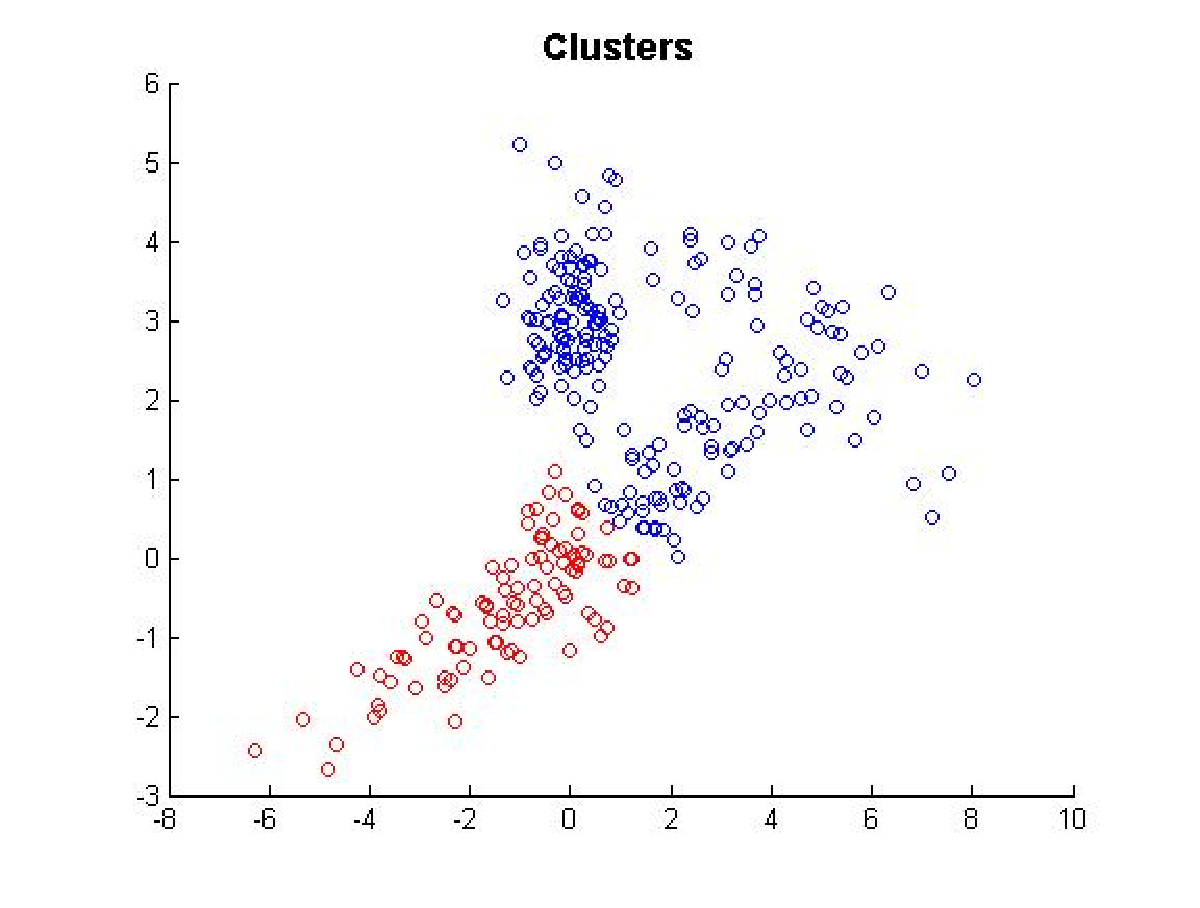
\includegraphics[scale=0.60]{imagens/tecnicas/clusters.eps}
\caption{Clusters gerados pelo K-Means}
\label{fig:clusters}
\end{figure}

Após a clusterização, é necessário associar cada cluster a uma classe. Para fazer isso, foi obtido o centróide de cada cluster e a média das amostras de cada classe. Com os centróides e as médias, o grupo com centróide mais próximo da média da Classe 1, foi associada a esta classe. O grupo com centróide mais distante da média da Classe 1, foi associado à Classe 2.

Os resultados obtidos estão representados na tabela \ref{tab:erro-kmeans}.

\begin{table}[H]
\begin{center}
\begin{tabular}{|l|l|l|l|}
\hline
Erro Global	&	Erro da Classe 1	&	Erro da Classe 2	&	Rand Corrigido	\\
\hline %----- linha horizontal
	0.18	&		0.36		&		0.00		&	0.4079		\\
\hline
\end{tabular}%--- fechamento do ambiente tabular
\end{center}   %fim da centralização da tabela
\caption{Tabela da taxa de erro do K-Means}
\label{tab:erro-kmeans}
\end{table}

Como existe sobreposição entre as distribuições, e a Classe 2 é multi-modal, o K-means encontra uma certa dificuldade em separar o conjunto em apenas 2 grupos. Pode-se observar também que, apesar de a taxa de erro global estar abaixo de 20\%, o Index de Rand Corrigido esteve mais próximo de uma categorização randomica do que de uma categorização perfeita, estando na região intermediária, próxima de 50\%.

\subsection{Máxima Verossimilhança e Algoritmo EM}
\label{subsec:exp-mle-em}

Nesta subseção, as estimativas de $P(\omega_i | x_k, \theta_i)$ foram feitas de formas diferentes para as duas classes. Para Classe 1, foi utilizado o Método da Máxima Verossimilhança, supondo uma normal multivariada. Já para a Classe 2 foi utilizado o algoritmo EM, supondo uma mistura de duas distribuições normais.

Para a Classe 1, obteve-se o vetor de média amostral e a matrix de covariância amostra, conforme as equações \ref{eq:mle_mean_normal} e \ref{eq:mle_sigma_normal}, respectivamente. Com estes parâmetros, foram calculados os valores das densidades para cada padrão de teste.

Já para a Classe 2, por se tratar de uma distribuição multimodal, foram calculados vetor de média amostral de cada compona e a matriz de covariância de cada componente. Isto foi feito por meio do \textit{Expectation-Maximization}. A partir destes parâmetros, foi calculada os valores da função de densidade para os padrões de teste de cada componente.

Uma vez com as funções de densidade de cada componente, a função densidade resultante foi calculada como a soma das funções de densidade de probabilidade das componentes ponderada pelas respectivas probabilidades a priori. Estas probabilidades a priori foram encontradas observando-se as proporções dos padrões de teste encontradas em cada distribuição da mistura.

Por fim, visto que a probabilidade a priori das classes são iguais, a regra de classificação se reduz a atribuir um padrão à classe de maior densidade de probabilidade seja maior para o padrão em questão.

Os resultados estão descritos na tabela abaixo:

\begin{table}[H]
\begin{center}
\begin{tabular}{|l|l|l|}
\hline
Erro Global			&	Erro da Classe 1	&	Erro da Classe 2	\\
\hline %----- linha horizontal
0.031 $\pm$ 0.015	&	0.051 $\pm$ 0.026	&	0.010 $\pm$ 0.013	\\
\hline
\end{tabular}%--- fechamento do ambiente tabular
\end{center}   %fim da centralização da tabela
\caption{Tabela da taxa de erro do MLE e EM combinados}
\label{tab:erro-mle-em}
\end{table}

\subsection{Janela de Parzen}
\label{subsec:exp-janeladeparzen}

Para estimar a função de densidade de probabilidade dos padrões de teste, foi considerada a Função de Kernel Gaussiana centrada em cada padrão de teste, com variância igual ao tamanho da janela $h$.

A forma utilizada para estimar a função de densidade, está expressa na equação \ref{eq:parzen_densidade}.

\begin{equation}
\label{eq:parzen_densidade}
\hat{p}(x) = \dfrac{1}{n} \dfrac{1}{h_1 \ldots h_p} \sum_{i = 1}^{n}\prod_{j = 1}^{p} K_j \left (\dfrac{x_j - x_{ij}}{h_j} \right )
\end{equation}
onde Kernel Gaussiano utilizado foi
\begin{equation}
\label{eq:kernel}
K_j(t) = \dfrac{1}{\sqrt{2\pi}} e^{- \dfrac{t^2}{2}}, t = \left (\dfrac{x - x_i}{h_n} \right)
\end{equation}

Conforme mencionado na seção \ref{subsec:janeladeparzen} é muito importante escolher a largura da janela adequada. Foram considerados valores independentes para largura da janela em cada dimensão. Para tal, o algoritmo foi executado 50 vezes para cada combinação de larguras de janelas pertencentes ao intervalo [0.1, 0.2, 0.3, ..., 9.8, 9.9, 10] e compondo o gráfico de superfície da figura \ref{fig:sup_parzen}. Nesta figura o eixo vertical representa o erro global médio, e os demais eixos representam combinações de valores da Janela.

\begin{figure}[H]
\center
\includegraphics[scale=0.60]{imagens/resultados/globalErrorsPerHValue.eps}
\caption{Gráfico de erro global por larguras de janela}
\label{fig:sup_parzen}
\end{figure}

Assim, escolheu-se um dos valores que estão na região de menor erro global, e os valores escolhidos foram 10 e 5 para o primeiro e o segundo atributo, respectivamente.

Novamente, como a probabilidade a priori é a mesma para ambas as classes, a decisão se resume a classificar o padrão como sendo da classe de maior densidade de probabilidade. tabela \ref{tab:erro-janela-parzen} mostra os erros obtidos por este classificador.

\begin{table}[H]
\begin{center}
\begin{tabular}{|l|l|l|}
\hline
Erro Global			&	Erro da Classe 1	&	Erro da Classe 2	\\
\hline %----- linha horizontal
0.024 $\pm$ 0.013	&	0.032 $\pm$ 0.021	&	0.017 $\pm$ 0.020	\\
\hline
\end{tabular}%--- fechamento do ambiente tabular
\end{center}   %fim da centralização da tabela
\caption{Tabela de erro da Janela de Parzen}
\label{tab:erro-janela-parzen}
\end{table}

\subsection{KNN}
\label{subsec:exp-knn}

Como visto na seção \ref{subsec:knn} a estimativa de probabilidade a posteriori se dá pela proporção de amostras de cada classe, $K_i$, dividido pelo número de vizinhos considerados, $K$, de acordo com a equação \ref{eq:knnposteriori}.

Assim como para o classificador baseado na Janela de Parzen, é preciso determinar o parâmetro $K$ adequado. Após testes exaustivos, concluiu-se que o valor de $K$ pouca varia a partir do $K$ = 3, para partição de testes utilizada. Portanto, o valor de $K$ escolhido para avaliação e comparação, foi $K$ = 3.

O algoritmo foi executado 50 vezes, e segue a tabela \ref{tab:erro-knn} mostra os resultados obtidos.

\begin{table}[H]
\begin{center}
\begin{tabular}{|l|l|l|}
\hline
Erro Global			&	Erro da Classe 1	&	Erro da Classe 2	\\
\hline %----- linha horizontal
0.030 $\pm$ 0.012	&	0.037 $\pm$ 0.024	&	0.024 $\pm$ 0.023	\\
\hline
\end{tabular}%--- fechamento do ambiente tabular
\end{center}   %fim da centralização da tabela
\caption{Tabela de erro do KNN}
\label{tab:erro-knn}
\end{table}

\subsection{Combinação de Classificadores}
\label{subsec:exp-combinacaodeclassificadores}


Para o classificador baseado em combinação, utilizou-se a regra da soma para estimativa da probabilidade a posteriori das classes.





